\chapter{Teoría de los \textsc{endus}}

Los ultrasonidos son ondas acústicas de naturaleza mecánica o elástica como
los sonidos. A diferencia de las ondas sónicas los ultrasonidos se
encuentran en una banda de frecuencia superior. Dicha banda parte de los 20
kHz y, carente de un límite físico, llega hoy hasta los 1000 MHz debido a
limitaciones tecnológicas. Las frecuencias empleadas en los ensayos no
destructivos se encuentran entre los 20 kHz y los 25 MHz. Cabe remarcar que
las propiedades de las ondas acústicas se mantienen invariantes con la
frecuencia, y por tanto, son comunes dentro del espectro acústico.

Las ondas ultrasónicas son perturbaciones mecánicas que viajan a través de
un medio elástico, por tanto, la condición primordial para que las ondas
ultrasónicas se propaguen a través de un medio es que este contenga
fracciones de materia tales como átomos o moléculas susceptibles de vibrar.
El medio determina también que modos de propagación pueden adoptar las
ondas ultrasónicas que se propagan a su través. Frecuentemente se asocia un
nombre característico a las ondas ultrasónicas en función del modo en el
que se propagan por el medio. A continuación se exponen los modos de
propagación de mayor relevancia.

\begin{itemize}
	\item Las \emph{ondas longitudinales}, también llamadas \emph{ondas
		de presión o compresión}, son aquellas que oscilan en la
		dirección de propagación. Al contrario que el resto de
		modos de propagación que sólo se dan en sólidos, el modo
		longitudinal puede estar presente también en líquidos y
		gases.
	\item En las \emph{ondas transversales o de cizalladura} las
		oscilaciones se producen en la dirección perpendicular a la
		dirección de propagación.
	\item Las \emph{ondas de superficie} se propagan únicamente a
		través de sólidos semi"=infinitos cuya superficie sea plana
		o curva y siempre siguiendo las irregularidades del
		contorno del mismo.
	\item Las \emph{ondas de Lamb o de chapa} son propias de medios
		sólidos en los que el espesor es del mismo orden que la
		longitud de onda, provocan la vibración de todo el
		material.
\end{itemize}

La energía acústica que se propaga por un medio se manifiesta en forma de
presión acústica, esta a su vez define el campo acústico. La presión
acústica se define como:

\begin{equation}
	p = Z\cdot v
	\label{eq:acuospressure}
\end{equation}

Ecuación en la que $v$ representa la velocidad de vibración y $Z$ la
impedancia acústica. La impedancia acústica es una medida de con que
resistencia se oponen los elementos de masa de un medio a la vibración
provocada por las ondas acústicas, en ningún caso da una relación de la
resistencia con la que el medio se opone a la propagación de la onda
acústica. Es una constante del medio que aumenta con la cohesión de sus
moléculas, y puede expresarse en función de la densidad $\rho_0$ y de la
velocidad de propagación de las ondas ultrasónicas en dicho medio $c$.

\begin{equation}
	Z = \rho_0\cdot c
	\label{eq:Zacoustic}
\end{equation}


\section{Campo acústico generado por un transductor de
ultrasonidos}\label{sec:field}

La excitación eléctrica de un transductor produce una onda de presión que
se propaga en el medio siguiendo las leyes físicas de la propagación de
ondas y, en particular, los principios de superposición de
Huygens\footnote{El tratamiento que se da en esta sección a los
transductores de ultrasonidos es similar al que la teoría de antenas da a
las antenas de apertura conocidas como bocinas. Para un mayor detalle
consultar el texto de Stutzman y Thiele, \cite{stutzman1997atd}.}. Se
denomina campo acústico a la distribución temporal y espacial de la presión
acústica a la que se someten las partículas materiales del medio en el que
se propagan las ondas acústicas. Las características del campo acústico
dependen principalmente de aspectos geométricos del transductor.

La región del campo acústico más próxima al transductor se conoce como
campo próximo o cercano. También recibe el nombre de campo de interferencia
debido a que en esa región el campo está constituido por máximos y mínimos
que surgen como resultado de las interferencias que se producen entre las
señales originadas en los distintos puntos del transductor. El máximo
principal del campo acústico delimita la región de campo próximo. La
longitud de esta región puede calcularse a partir del diámetro del
transductor $D$, o en su defecto a partir de la dimensión principal de
este.

\begin{equation}
	L_0 = \frac{D^2}{4\lambda}
	\label{eq:nearfield}
\end{equation}

Más allá del campo cercano encontramos el campo lejano. En el campo lejano
el frente de ondas de la radiación acústica empieza a divergir. Se llama
ángulo de divergencia del haz a la razón con la que el haz se expande y se
emplea el símbolo $\gamma_0$ para representarla. Puede calcularse
$\gamma_0$ a partir de la siguiente expresión.

\begin{equation}
	\sin{\gamma_0} = 1.2\cdot\frac{\lambda}{D}
	\label{eq:Adivergence}
\end{equation}

\begin{figure}
	\begin{center}
		\includegraphics{gis-pfc-ch5-01.mps}
	\end{center}
	\caption[Campo acústico generado por un transductor
	cilíndrico]{Diagrama simplificado que muestra el campo acústico
	generado por un transductor cilíndrico.}
	\label{fig:transceiver}
\end{figure}

En la \vref{fig:transceiver} el lector puede observar una representación
del campo acústico generado por un transductor de ultrasonidos cilíndrico.
Puede observarse la forma geométrica del campo próximo tal y como se ha
considerado en este documento: un cilindro de radio igual al del
transductor y altura $L_0$. En el interior del cilindro el campo acústico
permanece constante y en el exterior el campo es nulo. A continuación se
ilustra como el frente de ondas diverge en el campo lejano. La figura
empleada para representar el campo lejano es un tronco de cono en cuyo
interior el campo acústico iría incrementando de la superficie al eje.

Para finalizar este punto cabe mencionarse que el transductor es
responsable de que una determinada región de los materiales inspeccionados
no pueda ser caracterizada mediante el uso de ultrasonidos. La razón es que
tras emitir un pulso acústico un transductor no cesa inmediatamente de
vibrar, si no que lo sigue haciendo durante cierto tiempo a su frecuencia
natural de oscilación con un factor de amortiguamiento que depende de
factores constructivos. A la región del material que no puede ser
inspeccionada se la conoce como zona muerta o zona ciega. La zona ciega de
un material empieza en la superficie que está en contacto con el
transductor y su profundidad depende de la duración de los pulsos
acústicos.


\section{Técnicas empleadas en las inspecciones ultrasónicas, en
\protect{\textbf{\textsc{endus}}}}\label{sec:technics}

Atendiendo a la situación del receptor en los ensayos no destructivos
mediante ultrasonidos se distinguen dos técnicas: la técnica de pulso"=eco
y la técnica de transmisión. En la técnica de pulso"=eco el receptor suele
encontrarse cercano al emisor, de hecho es frecuente que un mismo
transductor haga las veces de emisor y receptor. Por el contrario en la
técnica de transmisión el receptor se coloca alineado en el eje del emisor
pero en el extremo opuesto del material inspeccionado.

\begin{figure}
	\begin{center}
		\subfloat[Inspección ultrasónica por transmisión]{
			\includegraphics{gis-pfc-ch5-02.mps}}
			\vspace*{.1\textheight}
		\subfloat[Inspección ultrasónica por pulso"=eco]{
			\includegraphics{gis-pfc-ch5-03.mps}}
	\end{center}
	\caption[Técnicas empleadas en ensayos no destructivos mediante
	ultrasonidos]{Diferencias en cuanto al número y posición de los
	transductores según la técnica empleada en una evaluación mediante
	ultrasonidos.}
	\label{fig:technics}
\end{figure}

Al propagarse un pulso acústico por el medio, parte de éste se refleja al
encontrarse con discontinuidades en la impedancia acústica, otra parte
seguirá avanzando hasta atravesar el material o verse completamente
atenuada. La señal que capta el receptor depende de su ubicación. De este
modo la señal recibida cuando la técnica empleada es la de pulso"=eco es la
suma de los pulsos reflejados o ecos. Si la técnica utilizada es la técnica
de transmisión se percibe el pulso original, modificado por haber
atravesado el medio. La información que contiene la señal recibida es, por
tanto, diferente.

La técnica de pulso"=eco se centra en el estudio de la amplitud, forma y
posición temporal de los ecos. La técnica de transmisión por su parte
observa posibles cambios de velocidad en el pulso acústico y mide la
atenuación que éste experimenta al pasar a través del medio. La información
que proporciona el estudio de los ecos es más rica pero también más
compleja. Por consiguiente la elección de una u otra técnica está
supeditada no sólo a las posibilidades de inspección que ofrece el medio,
si no también al tipo de información que se pretende obtener con el ensayo.


\section{Parámetros de calidad en una inspección}\label{sec:quality}

Los parámetros de calidad proporcionan una medida cualitativa de la bondad
de un ensayo. Los más empleados son resolución, linealidad y relación señal
a ruido.

En ensayos no destructivos la resolución es la distancia mínima (o una
medida en relación con ésta) a la que deben encontrarse dos singularidades
cercanas para que ambas sean detectadas distinguiéndose una de la otra. Se
hace distinción entre resolución axial y resolución lateral. La primera
alude a la distancia que debe haber entre dos singularidades alineadas en
la dirección longitudinal de propagación de las ondas acústicas, la segunda
a la que debe haber entre singularidades que se encuentren dispuestas en
una línea normal a esa dirección.

Atendiendo a la definición de resolución que se ha proporcionado, se
considera que la resolución es mejor si la distancia mínima disminuye y
peor si ésta aumenta. Teniendo esto en cuenta, para mejorar la resolución
axial de un sistema es necesario emplear dispositivos de banda ancha y
emitir pulsos estrechos de alta frecuencia. La frecuencia de los pulsos
acústicos está limitada por el espesor del medio, a medida que aumenta la
frecuencia disminuye la profundidad de penetración del pulso, resulta pues
conveniente adoptar una solución de compromiso.

La resolución lateral depende también de la frecuencia del pulso, es mejor
a medida que aumenta la frecuencia puesto que disminuye la longitud de
onda. Además depende del diámetro de los transductores, es peor cuanto más
anchos son éstos. Y en la región de campo lejano, la resolución lateral
empeora a medida que aumenta la profundidad.

El comportamiento de la resolución lateral con respecto al diámetro del
transductor y la frecuencia del pulso acústico transmitido, descrito en el
párrafo anterior puede deducirse de las ecuaciones
\cref{eq:nearfield,eq:Adivergence}. Puede observarse que, a medida que
aumenta la frecuencia y disminuye la longitud de onda del pulso, aumenta la
longitud de la región de campo cercano. En dicha región el campo acústico
se encuentra contenido en un cilindro de radio el del transductor, como ya
se ha mencionado, y a partir de ahí empieza a divergir según una razón que
disminuye con la longitud de onda. Para una mejor resolución es pertinente
que la región activa del campo ultrasónico sea lo más estrecha posible, de
ese modo se evita en la medida de lo posible que dos anomalías cercanas
queden cubiertas por el haz en un mismo evento de la secuencia de barrido.
Por tanto, se confirma por medio de estas ecuaciones los beneficios en
términos de resolución que redundan del uso de transductores de diámetro
estrecho y de pulsos ultrasónicos de alta frecuencia.

La definición y comportamiento de linealidad y relación señal a ruido son
los habituales en términos de sistemas electrónicos, por eso se entiende
que el lector tiene una noción al respecto y no se dan más aclaraciones en
este apartado.


\section{El problema del ruido en las inspecciones}\label{sec:noise}

La principal limitación en las inspecciones ultrasónicas es el ruido. Los
ensayos de este tipo se ven afectados generalmente por varias fuentes de
ruido. Según su naturaleza estadística el ruido perjudica en mayor o menor
medida los resultados de un ensayo. Cuanto más se asemeje el ruido a la
señal desde el punto de vista estadístico más la perjudicará y más difícil
será contrarrestar su efecto. El \emph{ruido incoherente aleatorio} tiene,
como su propio nombre indica, un origen aleatorio, y en consecuencia no
está relacionado con la señal. Por el contrario, los mecanismos que
originan el \emph{ruido coherente} son con frecuencia los mismos que dan
lugar a la señal de interés, y de ahí que exista una fuerte relación entre
el carácter estadístico de ambas señales.

Entre los exponentes más comunes de ruido incoherente aleatorio encontramos
el \emph{ruido gaussiano} y el \emph{ruido impulsivo}. El primero es
inherente a los equipos electrónicos y su origen es térmico, el segundo
tiene origen en las interferencias electromagnéticas causadas por equipos
eléctricos situados en las proximidades del sistema empleado para el
ensayo. Este tipo de ruido puede ser combatido sin dificultad con técnicas
bien conocidas como son: el promediado temporal de señales, el filtrado
paso-banda, la autocorrelación o las técnicas de compresión de pulsos, en
el caso del ruido gaussiano; y algoritmos de filtrado no lineal, en el caso
del ruido impulsivo.

En ensayos no destructivos mediante ultrasonidos, la señal de interés y el
\emph{ruido estructural o de grano} tienen una misma procedencia. Ambas
señales surgen como consecuencia de interactuar un pulso acústico con los
distintos elementos de que se compone un material. En el caso de la primera
de las señales, el pulso se refleja en las posibles particularidades
presentes en el medio como grietas o hendiduras. En el caso del ruido, las
reflexiones se producen al encontrarse el pulso con las partículas
suspendidas en el medio y de que éste se compone. Las diferencias entre
ambas señales radican en el tamaño y distribución de los elementos
reflectantes en el medio. Los reflectores que provocan el ruido son de
tamaño inferior a la longitud de onda de la señal propagada, y se
encuentran cercanos entre sí dispuestos de forma aleatoria por el medio.
Esto provoca que el carácter de la señal que aquí se ha bautizado como
ruido estructural sea, a efectos de una inspección ultrasónica, aleatorio e
impredecible. Si bien, la naturaleza de estas señales es similar y en
concreto lo es su naturaleza estadística. Por eso el ruido estructural es
considerado un ruido de tipo coherente y resulta complicado neutralizar su
efecto en los resultados del ensayo. Aún más, este ruido es el principal
factor limitante en ensayos de este tipo, enmascarando detalles en la señal
de interés que aportan información sobre posición, tamaño y forma de las
singularidades que son objeto de estudio. En contraposición a este hecho,
es posible emplear esta señal, que aquí es indeseada y considerada ruido,
en otro tipo de trabajos con el objetivo de caracterizar las propiedades
acústicas de un material.


\section{Fundamentos físicos del ruido estructural}

El ruido estructural es una consecuencia directa de la dispersión. Cuando
un frente de ondas incide sobre una partícula de tamaño comparable a su
longitud de onda, la energía que transporta se dispersa por la acción de
esa partícula. Dicha partícula actúa como un reflector esférico y selectivo
en frecuencia ---afectando más a las altas frecuencias\footnote{Según la
relación $c = \lambda\cdot f$, si se mantiene $c$, a medida que aumenta $f$
disminuye la longitud de onda y, por tanto, el tamaño de la partícula con
respecto a la longitud de onda aumenta.}--- que refleja la señal en todas
direcciones. De este modo, aquellos materiales que contienen un número
considerable de partículas susceptibles de interferir del modo descrito en
la propagación de un determinado frente de ondas, son considerados
materiales dispersivos.

En el caso de un frente de ondas acústicas que incide sobre un determinado
material dispersivo, la energía que tras el proceso de reflexión se propaga
en sentido contrario al sentido de propagación del frente de ondas se
conoce como \emph{back-scattering}. Por su parte, la energía perturbada por
la acción del reflector que continúa propagándose en el mismo sentido suele
denominarse \emph{forward-scattering}. En los \sig{endus} dependiendo de la
técnica empleada es uno u otro tipo de dispersión el que causa un mayor
deterioro de los resultados: si la técnica empleada es de pulso"=eco, el
\emph{back-scattering} será el más perjudicial; si, por el contrario, se
está empleando la técnica de transmisión, será el \emph{forward-scattering}
el más nocivo para el proceso.

Para poder estudiar el efecto del ruido estructural en las inspecciones
ultrasónicas de forma adecuada es necesario caracterizar el proceso de
emisión"=recepción que se da en un ensayo mediante ultrasonidos desde el
punto de vista de la respuesta al impulso o régimen transitorio.


\subsection{Análisis del proceso de emisión-recepción}

Los diferentes elementos que intervienen en el proceso de
emisión"=recepción de que consta una inspección ultrasónica tienen un
comportamiento lineal, esto permite estudiar todo el conjunto como un
sistema lineal, y ello a su vez posibilita el uso de técnicas propias del
análisis de este tipo de sistemas.

Supóngase un transductor de perfil arbitrario, al excitarse con un pulso
eléctrico, $u(t)$, y dadas a sus propiedades electromecánicas, emite un
pulso acústico de velocidad $v(t)$ relacionado con la respuesta impulsiva
de emisión del transductor, $h_{te}(t)$.

\begin{equation}
	v(t) = h_{te}(t)\otimes u(t)
	\label{eq:emiter}
\end{equation}

La respuesta impulsiva electrodinámica en emisión, $h_{te}(t)$ depende del
circuito electrónico empleado para excitar el transductor y de los
parámetros de diseño de este último.

La presión en un punto situado en el eje $y$ y a una distancia $z$ del
transductor es el resultado de la suma coherente de las aportaciones de
cada uno de los puntos que forman la cara del transductor por la que emite
la onda acústica, considerándolos como emisores omnidireccionales y
esféricos. La presión en cada punto del espacio está relacionada con la
velocidad en la cara del pistón por medio de la siguiente expresión:

\begin{equation}
	p(z, t) = \rho\,\frac{\partial}{\partial t}\left\{v(t)\otimes
	h_{m}(z, t)\right\}
	\label{eq:diffracpressure}
\end{equation}

Siendo $\rho$ la densidad del medio por la que se propaga la onda acústica
y $h_{m}(z, t)$ la respuesta al impulso en el medio de propagación
considerando la difracción que se produce en dicho medio.

La propagación de una onda acústica se ve sometida a fenómenos de
difracción propios de la naturaleza ondulatoria de la radiación acústica y
fenómenos de atenuación a consecuencia de la interacción con el medio. De
cara al estudio de la propagación de la onda estos fenómenos pueden
tratarse por separado. Por un lado se considera el efecto de la difracción
sobre la onda en un medio homogéneo y sin pérdidas, y por otro la
atenuación que induce el medio. Esta aproximación mantiene su validez
siempre que el estudio afecte a una región del campo muy próxima al
transductor. Si se considera esta aproximación, y se tiene $h_d(z, t)$, la
respuesta al impulso en un medio homogéneo y sin pérdidas a la difracción,
y $a(z, t)$, la atenuación atribuida al medio; puede descomponerse la
respuesta al impulso en el medio de propagación a la difracción en esos dos
términos:

\begin{equation}
	h_m(z, t) = h_d(z, t)\otimes a(z, t)
	\label{eq:diffraction}
\end{equation}

La atenuación es selectiva en frecuencia y ello se asocia a los siguientes
aspectos derivados de la existencia de una macro y una micro"=estructura en
el material:

\begin{itemize}
	\item La absorción o transformación de la energía acústica que
		transporta la onda en calor.
	\item Y los efectos de dispersión de la energía.
\end{itemize}

La expresión que define la atenuación sufrida por la onda acústica toma la
siguiente forma a partir de $\alpha(\omega)$ o coeficiente de atenuación
característico del medio.

\begin{equation}
	A(z, \omega) = e^{\int^z_0 -\alpha(z, \omega)dz} 
	\label{eq:loss}
\end{equation}

Cuando la onda acústica incide sobre un reflector, las características de
éste determinan la relación entre la onda incidente y la reflejada. Esta
relación viene dada por la función de reflectividad, $h_r(t)$, que depende
de la frecuencia de la onda de presión. Si la reflexión que se produce al
llegar la onda hasta la partícula es especular, $h_r(t)$ coincide con una
delta de Dirac ponderada.

Como consecuencia de la reflexión, una señal distinta de la emitida por el
transductor en origen regresa a éste. Por tanto, se produce en la cara del
transductor que da al material una presión variable con el tiempo $p_R(z,
t)$, constituida por la suma de la presión que se produce en cada punto de
la mencionada superficie.

\begin{equation}
	p_R(z, t) = p(z, t)\otimes h_r(t)\otimes h_m(z, t)
	\label{eq:recpressure}
\end{equation}

Del mismo modo, parte de la señal reflejada avanza en el mismo sentido de
propagación que la onda incidente. Si no es dispersada completamente en el
medio avanza hasta atravesar el material por completo. En ese caso, si es
la técnica de transmisión la técnica empleada, una presión semejante a
$p_R(z, t)$ se produce en la cara del transductor que se encuentra al otro
extremo del material. La función de reflectividad no varía, tan sólo cambia
la distancia que debe atravesar el frente de ondas hasta alcanzar el
transductor y, por tanto, es diferente la contribución de la respuesta al
impulso en el medio a la difracción, $h_m(z^\prime, t)$ en el segundo
trayecto.

Finalmente, la presión $p_R$ se traduce en una señal eléctrica en bornes
del transductor. Esta señal está relacionada con la respuesta impulsiva del
transductor en recepción, $h_{tr}(t)$, que depende, al igual que
$h_{te}(t)$ del circuito acondicionador y del proceso de fabricación del
transductor.

\begin{equation}
	y(t) = h_{tr}(t)\otimes p_R(z, t)
	\label{eq:receiver}
\end{equation}

Por consiguiente el proceso de emisión"=recepción en el que se fundamentan
los \sig{endus} puede describirse mediante la respuesta impulsional en
cascada de todos los fenómenos descritos.

\begin{equation}\label{eq:emirec}
	\begin{split}
		y(t) = \rho_0\frac{\partial}{\partial t}\{u(t)& \otimes
		h_{te}(t)\otimes h_d(z, t)\otimes a(z, t)\otimes \\
		&\otimes h_r(t)\otimes h_d(z, t)\otimes a(z, t)\otimes
		h_{tr}(t)\}
	\end{split}
\end{equation}

La \vref{fig:emirecmodel} muestra un diagrama de bloques que representa el
proceso de emisión"=recepción y todos los fenómenos que en el intervienen
según el modelo empleado en este documento. La función de transferencia del
sistema puede obtenerse de modo sencillo aplicando el teorema de la
convolución.

\begin{figure}
	\begin{center}
		\includegraphics[scale=1, keepaspectratio=true]%
		{gis-pfc-ch5-04.mps}
	\end{center}
	\caption[Proceso de emisión"=recepción y elementos que en él
	intervienen]{Diagrama de bloques que representa el proceso de
	emisión"=recepción y todos los elementos que en el intervienen
	(considerando el modelo propuesto).}
	\label{fig:emirecmodel}
\end{figure}

\begin{equation}
	\begin{split}
		Y(\omega) = j\omega\rho_0& \cdot U(\omega)\cdot
		H_{te}(\omega)\cdot H^2_d(z, \omega)\cdot
		A^2(z, \omega)\cdot \\
		&\cdot H_r(\omega)\cdot H_{tr}(\omega)
	\end{split}
	\label{eq:transference}
\end{equation}

Aprovechando la linealidad del sistema se agrupan los términos de la
función de transferencia en \eqref{eq:groupedtransference}, para que el
resultado quede en función de la respuesta electromecánica del transductor,
$X(\omega)$, y de la respuesta espacial al impulso, $H(z, \omega)$.

\begin{equation}
	Y(\omega) = X(\omega)\cdot H(z, \omega)\cdot A^2(z, \omega)
	\label{eq:groupedtransference}
\end{equation}

\begin{equation}
	X(\omega) = j\omega\rho_0\cdot U(\omega)\cdot H_{te}(\omega)\cdot
	H_{tr}(\omega)
	\label{eq:transducer}
\end{equation}

Siendo esta última, la respuesta espacial al impulso, función de la
posición del reflector y de su forma, o lo que es lo mismo, de las
funciones de reflectividad y difracción.

\begin{equation}
	H(z, \omega) = H^2_d(z, \omega)\cdot H_r(\omega)
	\label{eq:spacialresponse}
\end{equation}

Al agrupar de este modo la función de transferencia se establece de forma
explícita la separación entre los procesos de difracción y atenuación.
Además es posible establecer nuevas separaciones: dejando por un lado los
efectos debidos a los transductores y electrónica de acondicionamiento,
$X(\omega)$; por otro la influencia del medio en la onda que se propaga, es
decir, la atenuación, $A(z, \omega)$; y, finalmente, por otro los efectos
de la propagación y la interacción con el reflector, $H(z, \omega)$.


\subsection{Atenuación en medios dispersivos}

La atenuación es el fenómeno en el que se manifiesta la influencia del
medio en la propagación de una onda. Suponiendo un medio en el que la
atenuación depende únicamente de la frecuencia de la onda acústica, puede
calcularse la atenuación sufrida por dicha onda tras haberse propagado una
distancia $z$ a lo largo del medio, como:

\begin{equation}
	A(z, \omega) = e^{-\alpha(\omega)\cdot z}
	\label{eq:independentloss}
\end{equation}

Donde, como se anticipó en \eqref{eq:loss}, $\alpha(\omega)$ es el
coeficiente de atenuación. Cuando el material por el que se propaga la onda
es no homogéneo, la atenuación se debe a dos fenómenos:

\begin{description}
	\item[Absorción] Fenómeno que también aparece en medios homogéneos
		y por el cual la energía que transporta la onda se
		transforma en otro tipo de energía, por lo general en
		calor.
	\item[Dispersión] En este estudio se entiende dispersión como la
		distorsión que ejerce sobre el frente de ondas el grano
		suspendido en el medio. La acción del borde del grano, así
		como los saltos de índice de refracción que provoca la
		presencia de ese grano en el medio, contribuyen a la
		aparición de este fenómeno.
\end{description}

En el coeficiente de atenuación global vienen reflejadas las acciones que
sobre la señal ejercen ambos fenómenos. Siendo $\alpha_s(\omega)$ la
contribución de la dispersión y $\alpha_a(\omega)$ la contribución de la
absorción.

\begin{equation}
	\alpha(\omega) = \alpha_a(\omega) + \alpha_s(\omega)
	\label{eq:losscoefficient}
\end{equation}

El coeficiente de absorción depende del cuadrado de la frecuencia a la que
oscila el frente de ondas, $\alpha_a(\omega) = a_1\omega^2$. Siendo $a_1$
la constante de absorción del material. Por su parte, $\alpha_s(\omega)$
depende del tamaño, forma, orientación y distribución de los granos en el
medio, aunque también de la frecuencia como se muestra a continuación.


\subsection{Estimación del coeficiente de dispersión para un material
dispersivo de naturaleza granulosa}

El coeficiente de dispersión de un material no homogéneo de naturaleza
granulosa puede estimarse de forma teórica asumiendo que los granos en el
medio forman una matriz tridimensional de pequeños reflectores o granos
esféricos, tal y como se muestra en la \vref{fig:matrix}. Asumiendo este
modelo, puede obtenerse la respuesta global del medio obteniendo la
respuesta de un reflector e integrando a todo el volumen el resultado
obtenido para un solo grano.

\begin{figure}
	\begin{center}
		\includegraphics[scale=1, keepaspectratio=true]%
		{gis-pfc-ch5-05.mps}
	\end{center}
	\caption[Modelo de pequeños receptores] {Modelo de pequeños
	receptores para la estimación del coeficiente de dispersión.}
	\label{fig:matrix}
\end{figure}

La \vref{eq:disperser} es una aproximación de la respuesta espacial al
impulso de un solo dispersor cuando sobre el incide un frente de ondas
ultrasónicas longitudinales plano. En esta ecuación se han empleado: $k$,
constante que depende de la geometría del reflector; la frecuencia angular
a la que oscila el frente de ondas, $\omega$; $c_l$, o velocidad a la que
se propaga el frente de ondas; $V$ volumen del dispersor; y $z$ distancia
entre éste y el transductor.

\begin{equation}
	H_s(z, \omega) = k\,\frac{V\omega^2}{zc^2_l}\,e^{-j2\omega z/c}
	\label{eq:disperser}
\end{equation}

De $H_s(z, \omega)$ se deduce que la onda reflejada es dependiente de la
frecuencia angular de oscilación. De hecho, se manifiestan las propiedades
de filtro paso bajo que muestra la partícula. Si el reflector es de tamaño
muy superior a la longitud de onda de la radiación acústica, la dependencia
de $H_s(z, \omega)$ con $\omega$ es en la práctica despreciable, y sólo
dependería de la geometría del reflector.

Si el conjunto de dispersores suspendidos en el medio es homogéneo, y todos
ellos están equiespaciados y presentan isotropía, es posible suponer que el
frente de ondas se encuentra de forma sucesiva y periódica con planos de
reflectores. Si se supone además que la contribución de la dispersión
múltiple es despreciable frente a la contribución de las reflexiones
primarias, el frente de ondas que se propaga tras el primer plano de
partículas es la suma vectorial de la onda no dispersada y de una pequeña
fracción de la onda que tras interactuar con dichas partículas sigue
propagándose en la misma dirección en la que se propaga el frente de ondas.
Si se tiene en cuenta el comportamiento de un plano de reflectores,
semejante a un filtro paso bajo, el resultado de la dispersión es \emph{un
frente de ondas que con respecto al original tiene atenuadas las altas
frecuencias}. Por tanto, puede manifestarse un equivalente, \emph{un
material dispersivo se comporta como un filtro paso bajo cuya
característica de atenuación depende de la profundidad que haya alcanzado
la onda en su propagación}.

Puede escribirse una expresión de la atenuación causada por la dispersión
si se considera ésta en función de la energía neta que aporta al frente de
ondas cada uno de los planos reflectores. Esta expresión queda en función
del diámetro del grano $D$, y de $s_1$, una constante de dispersión que
depende del material.

\begin{equation}
	A_s(z, \omega) = e^{-s_1D^3\omega^4z}
	\label{eq:dispersionloss}
\end{equation}

Mediante esta expresión y la \cref{eq:independentloss}, aplicando después
la \cref{eq:losscoefficient}, es posible calcular el coeficiente de
atenuación debido a la dispersión, $\alpha_s$, en la región de Rayleigh, en
la que $D\ll\lambda$. Empleando deducciones semejantes puede obtenerse el
coeficiente de atenuación en distintas situaciones de tamaño de grano y
longitud de onda.

{\setlength{\extrarowheight}{0.5ex}
\begin{equation}
	\alpha_s(\omega) = \left\{
	\begin{array}{c@{\qquad\text{---}\qquad}c@{\quad}c}
		s_1D^3\omega^4 & D\ll\lambda %
		& \text{(Región de Rayleigh)} \\
		s_2D\omega & D\simeq\lambda %
		& \text{(Región estocástica)} \\
		s_3/D & D>\lambda & \text{(Región de difusión)}
	\end{array}
	\right.
	\label{eq:dispersionlossreg}
\end{equation}}

\begin{figure}
	\begin{center}
		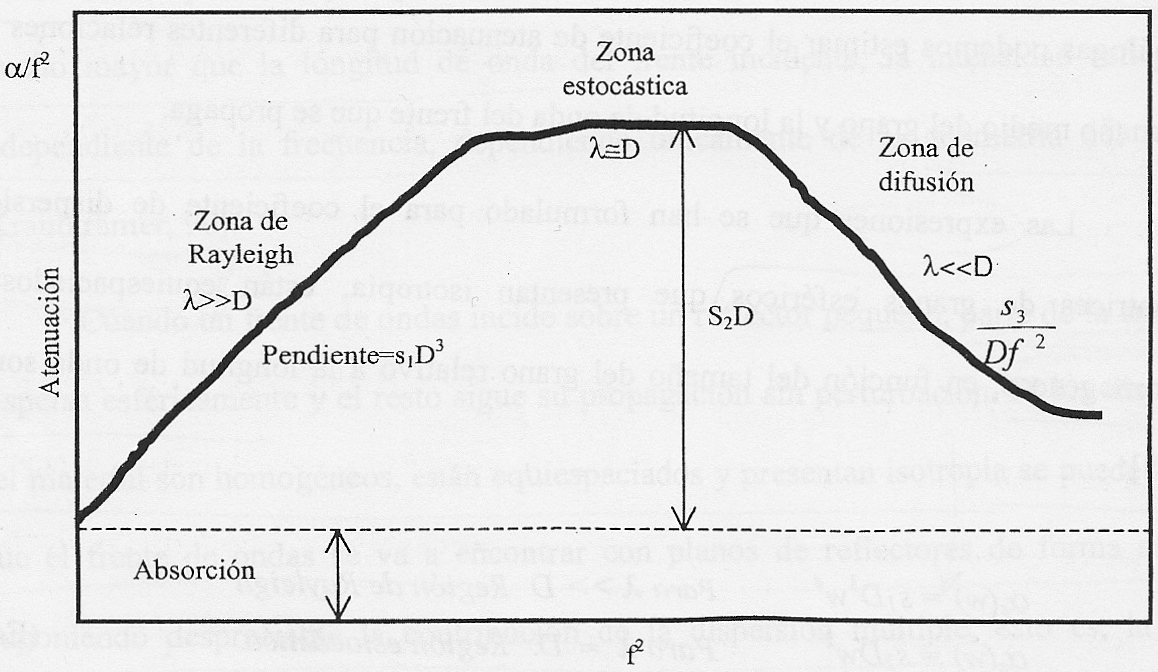
\includegraphics{gis-pfc-ch5-06.jpg}
	\end{center}
	\caption[Comportamiento del coeficiente de atenuación en las
	distintas regiones del medio]{Representación del coeficiente de
	atenuación que muestra su comportamiento en las distintas regiones
	del material.}
	\label{fig:losscoefficient}
\end{figure}

Para finalizar este apartado, en la \vref{fig:losscoefficient} se muestra
una representación del coeficiente de atenuación, en concreto del cociente
$\alpha/f^2$, con respecto al cuadrado de la frecuencia. En la gráfica es
posible apreciar el comportamiento del coeficiente de dispersión en cada
una de las regiones descritas, y como el término que introduce la absorción
es de valor constante con la frecuencia. La región de difusión muestra una
atenuación abrupta que responde a una exponencial decreciente descrita por
la expresión $s_3/(Df^2)$.


\subsection{Limitaciones impuestas por la dispersión en los ensayos
ultrasónicos}

La dispersión, que contribuye de dos modos distintos a perjudicar el
proceso de inspección ultrasónica, por un lado atenuando la señal acústica,
por otro lado causando el ruido de grano, es el principal factor limitante
en los ensayos no destructivos. Es habitual que la dispersión limite la
profundidad de una inspección a la región de Rayleigh.

Cualquier material posee granos de diferentes tamaños y, por tanto, un
frente de ondas acústicas que atraviesa un material se ve afectado por la
dispersión como si se encontrase en las tres regiones de dispersión
descritas. No obstante, es el grano de mayor tamaño el que en la práctica
determina el comportamiento del material en términos de dispersión.

La dispersión, debido a que es el causante del ruido estructural, no puede
contrarrestarse aumentando la potencia de la onda ultrasónica en emisión.
La solución primera para evitar la dispersión pasa por disminuir la
frecuencia de la onda, pero esto desemboca también en una pérdida de
resolución. La mejor alternativa consiste en emplear técnicas de
procesamiento de señal que reduzcan la energía del ruido estructural en
recepción.


\section{Algoritmos utilizados para la reducción del ruido estructural}

Dejando a un lado las técnicas empleadas en la eliminación de ruido
incoherente aleatorio, ineficaces por completo contra el ruido estructural,
existe un conjunto de métodos orientados a combatir este tipo de ruido.

Las técnicas empleadas con mayor frecuencia con el objeto de conseguir
mayor \sig{snr} en entornos en los que la presencia de ruido estructural es
notable son aquellas que aprovechan la diversidad de información hallada al
trabajar con señales incorreladas entre sí. Estas técnicas tratan de
obtener una señal con una mayor \sig{snr} a partir de la composición de
varias señales generadas mediante un mismo mecanismo pero de forma que la
medida de correlación entre cada una de ellas sea pobre. Los métodos
empleados más a menudo con tal propósito son:

\begin{itemize}
	\item Las técnicas que explotan la diversidad espacial, en las que
		básicamente se repite el mismo experimento variando cada
		vez la orientación de los transductores implicados en el
		mismo.
	\item Y las técnicas de diversidad frecuencial, manteniendo la
		posición de los transductores se repite el experimento
		utilizando señales situadas en una banda espectral
		diferente unas de otras.
\end{itemize}

Este tipo de técnicas consiguen mejorar de forma considerable la \sig{snr}
en inspecciones ultrasónicas, no obstante presentan una serie de
inconvenientes que las hacen inapropiadas en determinadas situaciones. Por
un lado, las técnicas de diversidad espacial se ven obstaculizadas con
frecuencia por las dimensiones y forma de las piezas evaluadas, siendo en
ocasiones imposible emplearlas. En cuanto a las técnicas de diversidad en
frecuencia, los transductores empleados en inspecciones ultrasónicas actúan
por lo común en una banda no lo bastante ancha como para poder dividirla en
un gran número de subbandas y así poder emitir suficientes señales
acústicas repartidas por el espectro de frecuencias. Para poder emplear una
técnica así serían necesarios varios transductores que emitiesen en bandas
de frecuencia señales acústicas con ancho de banda controlado y que todos
estuviesen situados en la misma posición.

La dificultad que conlleva implementar las técnicas anteriormente descritas
ha contribuido a la proliferación de técnicas que a partir de una única
traza sacan partido de las diferencias estadísticas que existen entre la
señal que procede de un defecto y el ruido estructural. Dentro de esta
categoría el algoritmo que ha alcanzado un éxito mayor y en consecuencia se
ha convertido en el paradigma de las técnicas de reducción de ruido
estructural se conoce como técnica de partición espectral o del inglés
\emph{Split Spectrum Processing} (\psig{ssp}) y fue en inicio propuesto por
Vernon Newhouse en 1982. El algoritmo está basado en la explotación de la
seudo"=diversidad frecuencial que existe entre las diferentes trazas de
banda estrecha que se obtienen al descomponer con un banco de filtros paso
banda la señal resultante tras un ensayo. No obstante los excelentes
resultados encontrados utilizando esta técnica, la gran sensibilidad que
muestra el algoritmo a la sintonía de los principales parámetros que
definen su comportamiento lo convierten en escasamente robusto. A
consecuencia de esto han aparecido numerosas publicaciones que se
circunscriben a proporcionar configuraciones del algoritmo que proporcionen
resultados óptimos, alternativamente aparecen también variaciones del
\sig{ssp} que persiguen mejorarlo. A pesar de su éxito, el \sig{ssp} no es
el único método empleado con el objetivo de sustraer el ruido de grano de
la señal de interés de un \sig{endus}. Otros trabajos incluyen, la
estimación de máxima verosimilitud, técnicas de filtrado paso"=banda que
eliminan la mitad superior del espectro de la señal, técnicas
tiempo"=frecuencia como son la transformada de Wigner"=Ville o las Wavelet,
técnicas que sacan partido de la información que aporta el retardo de
grupo, técnicas no lineales y, finalmente, técnicas de ruido residual.

A pesar del gran número de técnicas dedicadas a eliminar el ruido
estructural, son pocos los trabajos orientados a establecer una relación
entre ellas, a compararlas, a clasificarlas según su comportamiento en
distintos tipos de materiales o a justificar por qué el uso de una u otra
técnica.


\section{Técnicas de procesado por partición del espectro}

Bajo el término <<técnicas de procesado por partición del espectro>>, en
inglés \emph{Split Spectrum Processing Techniques}, o simplemente
\psig{ssp}, se reúnen una serie de algoritmos cuya aplicación es la
reducción del efecto del ruido estructural o de grano en los resultados de
un \sig{endus}. El principio en el que se fundamentan estas técnicas es
similar al que rige las técnicas de diversidad convencionales. A partir de
varias señales incorreladas entre sí se construye una señal cuya \sig{snr}
es considerablemente mejor que la \sig{snr} de cualquiera de las señales
primitivas por separado. Las técnicas de \sig{ssp}, a diferencia de las
técnicas basadas en la diversidad, consiguen sólo una seudo"=diversidad en
frecuencia a partir de una única traza de la señal que se obtiene tras un
\sig{endus}. Con frecuencia se obtienen buenos resultados empleando estas
técnicas lo que, sumado a la sencillez con la que puede implementarse un
experimento fundamentado en las mismas, recordando que no es requerida una
redundancia real basada en la utilización de varias señales, las ha
convertido en las técnicas más populares en el ámbito de los \sig{endus}. A
consecuencia de la reputación con la que se han visto revestidas
recientemente numerosas investigaciones se han llevado a cabo en las
décadas de los ochenta y los noventa, así como a principios de siglo, con
el fin de mejorar en la medida de lo posible los buenos resultados que ya
de por sí proporcionan las técnicas de \sig{ssp}.

El procedimiento (más detallado en el \cref{tab:sspfeatures}) que por lo
general sigue todo el conjunto de técnicas de \sig{ssp} consiste en aplicar
una transformación sobre la traza que comprende dos pasos:

\begin{itemize}
	\item El primero, dividir la traza en un número determinado de
		señales de banda estrecha, para lo que se emplea un banco
		de filtros.
	\item En segundo lugar se reconstruye la traza, o más bien una
		versión de ésta con una \sig{snr} mejorada, mediante un
		algoritmo de reconstrucción no lineal.
\end{itemize}

Las diferencias entre el carácter estadístico del ruido y de la señal
procedente del defecto hacen que el procedimiento anterior conduzca al
resultado deseado. Para concretar, la distribución de la energía del ruido
no es equitativa en frecuencia, de ahí que sea posible encontrar señales
incorreladas en ruido mediante la división espectral que realiza el banco
de filtros. Por otro lado, la linealidad que presenta la componente de la
señal ---o alteración de la misma según sea el caso--- originada en la
reflexión que se produce al encontrarse la onda acústica con el defecto
conlleva que la muestra que identifica la presencia del defecto se
encuentra en la misma posición en todas las trazas de banda estrecha. Los
métodos de \sig{ssp} aprovechan de manera implícita esta última
característica de la traza para magnificar la componente de la señal que
indica la presencia del defecto por lo que son catalogados en la
bibliografía como métodos que explotan la fase del defecto.


\begin{table}
	\centering
	\begin{tabulary}{.95\textwidth}{>{$(}c<{)$}Lr@{\hspace{6pt}}L}
		\toprule
		\multicolumn{2}{c}{Parámetros} %
		& \multicolumn{2}{c}{Algoritmo} \\
		\cmidrule(r){1-2}\cmidrule(l){3-4}
		y & Señal a procesar & 1. & Generar del banco de filtros \\
		f_\text{min} %
		& Frecuencia inferior de corte del banco de filtros & 2. %
		& Calcular la \sig{fft} de $y$ \\
		f_\text{max} %
		& Frecuencia superior de corte del banco de filtros & 3. %
		& Procesar el resultado obtenido en (2) con el banco de %
		filtros \\
		\Delta f & Separación entre filtros & 4. %
		& Calcular la \sig{ifft} de las trazas de banda estrecha \\
		pb & Ancho de banda de los filtros & 5. %
		& Normalizar la amplitud de las trazas de banda estrecha \\
		h_f & Tipo de filtro empleado & 6. %
		& Construir una única traza a partir de las trazas de %
		banda estrecha normalizadas \\
		\bottomrule
	\end{tabulary}
	\caption[Particularidades que en general se aplican a todos los
	algoritmos de \sig{ssp}]{Particularidades que en general se aplican
	a todos los algoritmos de \sig{ssp}.}
	\label{tab:sspfeatures}
\end{table}

\begin{figure}
	\begin{center}
		\includegraphics{gis-pfc-ch5-07.mps}
	\end{center}
	\caption[Parámetros de configuración del banco de filtros]%
	{Representación esquemática en la que pueden observarse los
	parámetros empleados en la configuración del banco de filtros
	comparados con el espectro de la señal de audio.}
	\label{fig:filter}
\end{figure}

La eficacia de las técnicas de \sig{ssp} no está garantizada, depende en
gran parte de dos de los parámetros listados en el \cref{tab:sspfeatures}.
Por un lado está la configuración del banco de filtros, a destacar dos
aspectos: el tipo de filtro empleado y la zona del aspecto en la que se
aplica el método. Según afirma M.\,A. Izquierdo (en \cite{garcia2000mrsr}),
trabajos realizados a principios de los noventa como los de P.\,Karpur
apuntan a la existencia de una relación entre el factor de forma de los
filtros que se utilizan para realizar la partición de espectro y la bondad
de los resultados aportados por la técnica de \sig{ssp}. Señala M.\,A.
Izquierdo que, a pesar de que la influencia que ejerce este parámetro en la
calidad del ensayo haya mostrado ser notable, estudios posteriores no han
tenido en cuenta las conclusiones alcanzadas por Karpur. La región del
espectro que queda bajo el banco de filtros puede configurarse ajustando
las frecuencias de corte superior e inferior del banco ---quedando
indirectamente condicionados el ancho de banda de los filtros y la
separación entre los mismos---. Es importante evitar que la banda de paso
del banco coincida con alguna porción de la señal en la que la información
espectral que indica la presencia del defecto quede enmascarada por el
ruido de grano. Cuando así ocurre la efectividad del método se reduce en
gran medida.

El parámetro que resta por considerar no es otro que el algoritmo de
reconstrucción que permite recuperar la traza definitiva. Las técnicas de
\sig{ssp} se basan en la estabilidad de la fase de ahí su precaria
robustez. El algoritmo de reconstrucción empleado es un factor determinante
del que depende en gran parte la robustez de la técnica. Por tanto, aplicar
un algoritmo de reconstrucción adecuado a las muestras es crucial para
obtener buenos resultados. Los algoritmos más empleados son el de mínimo
del ensamble y el del umbral de polaridad (\emph{Polarity Thresholding}) o
combinación de ambos, a continuación se citan otros.

Los trabajos mencionados en este apartado siguen todos una misma línea de
investigación, descubrir qué configuración del banco de filtros y qué
método de reconstrucción optimizan los resultados de aplicar las técnicas
de \sig{ssp} en un \sig{endus}. Se ha dicho que el término \sig{ssp} agrupa
a un conjunto de técnicas, lo que las diferencia precisamente es, o bien el
algoritmo de reconstrucción que emplean, o bien la forma en la que se
configura el banco de filtros, en ocasiones ambos. En cuanto a la
configuración del banco de filtros, algunos trabajos, es especial algunos
de Karpur, aportan avances significativos. El autor encuentra para el
algoritmo de mínimos, de forma analítica y apoyándose en un modelo
estacionario del ruido de grano, los parámetros que optimizan el
rendimiento de la técnica de \sig{ssp}. Los valores hallados son los
siguientes:

\begin{equation}
	\begin{split}
		N & = B\cdot T_y + 1 \\	
		b & = \Delta f = \frac{1}{T_y}
	\end{split}
\end{equation}

Donde $N$ representa el número óptimo de filtros, $B$ el ancho de banda del
transductor en el segmento de recepción, $T_y$ la duración de la señal
recibida, $b$ el ancho de banda de cada filtro, y $\Delta f$ la separación
entre filtros. Por otro lado Karpur afirma en otro de sus estudios, esta
vez apoyándose en la expresión para la atenuación en la región de Rayleigh,
que el banco de filtros debe aplicarse en las frecuencias más bajas del
espectro de la señal, ya que es en esa zona en la que se concentra la mayor
parte de la energía correspondiente a la radiación que tiene origen en el
defecto. Otros estudios utilizan la información relativa a la distribución
espectral de la \sig{snr}, obtenida mediante algoritmos como el del
histograma espectral o a partir de estadísticos del retardo de grupo como
p.e. la entropía móvil, para determinar cuál es la región del espectro de
la señal en la que es óptimo aplicar el filtrado.

En cuanto a los algoritmos de reconstrucción J.\,Saniie llega a la
conclusión, en su trabajo de 1991 en el que estudia los filtros de orden
aplicados como algoritmos de composición, de que los mejores resultados se
obtienen cuando la señal proviniente del defecto y el ruido estructural
están estadísticamente separados en un determinado cuantil. Dependiendo de
las distribuciones de probabilidad del ruido y del defecto, resulta
apropiado emplear algoritmos de mínimos, mediana o máximos del ensamble,
aunque por lo general el algoritmo de mínimos es el que mejores resultados
proporciona.

Por su parte M.\,G.\,Gustafsson propone una variante en el conjunto de las
técnicas de \sig{ssp} en la que, basándose en la teoría bayesiana de
detección y a partir de la información de la señal y el ruido coherente,
pueden encontrarse todos los parámetros necesarios para aplicar la técnica
de \sig{ssp}. El nombre que recibe usualmente esta variante es técnica de
\sig{ssp} con detección óptima.
